\report{Multi-object tracking на основе библиотеки Norfair}{Георгий Сичкар}

\subsection{Введение}
Доклад посвящен задаче multi-object-tracking, а также битблиотеке с открытым исходным кодом \textbf{norfair}. Это поверхностное погружение в предметную область трекинга объектов на видео. План доклада примерно такой:

\begin{itemize}
    \item базовые определения и терминология;
    \item гайд по использованию \textbf{norfair};
    \item примеры использования.
\end{itemize}

\subsection{Трекинг}
\emph{{Object tracking}}~--- это задача отслеживания объекта на протяжении всего видео.
\begin{itemize}
    \item Single object tracking (SOT)~--- обнаружение объекта не требуется (видеонаблюдение, видеотрансляции)
    \item Multi-object tracking (MOT)~--- одним из этапов является детектирование объектов (робототехника, автономное движение)
\end{itemize}

Существует довольно большое множество областей, в которых используется MOT:
\begin{itemize}
    \item cпортивный анализ~--- отслеживания мяча в теннисе, волейболе, футболе (\href{https://www.hawkeyeinnovations.com/}{Hawk-Eye Innovations});
    \item видеонаблюдение~--- отслеживание необычной активности (\href{https://www.hikvision.com/}{HIKVISION});
    \item робототехника~--- сложные взаимодействия (с человеком).
\end{itemize}

\subsection{Этапы трекинга}

Зачастую алгоритмы состоят из трех частей. Первый этап~--- это детекция объекта на кадре. Второй этап заключается в предсказании перемещения объекта на основе уже имеющихся данных. Ну если более понятным языком, то мы в системе храним какой-то пул объектов, которые распознали ранее, и по данным о их перемещениях в прошлом пытаемся угадать куда они попадут в будущем. После создания гипотезы "где могут находится объекты" на третьем шаге происходит сопоставление объектов которые мы распознали с предсказанными перемещениями.

\subsection{Алгоритмы и их реализации с открытым исходным кодом}

Существует множество алгоритмов для решения задачи MOT. Здесь приведен список нескольких довольно популярных вариантов:
\begin{itemize}
    \item SORT~--- использует Kalman-фильтр и Венгерский алгоритм
    \item DeepSORT~--- расширение SORT (дополнительно использует сверточную нейронную сеть, для определения идентичности объекта)
    \item ByteTrack
    \item FairMOT
\end{itemize}

Есть множество библиотек с открытым исходным кодом, которые реализуют MOT, опираясь на вышеописанные алгоритмы. Ниже перечислены самые популярные решения:
\begin{itemize}
    \item \href{https://opencv.org/}{OpenCV} (популярная библиотека для computer vision);
    \item \href{https://github.com/MVIG-SJTU/AlphaPose}{AlphPose} (используется для трэкинга людей);
    \item \href{https://github.com/davisking/dlib}{dblib} (только SOT);
    \item \href{https://docs.ultralytics.com/ru/modes/track/}{Ultralytics YOLO} (алгоритм трэкинга~--- ByteTrack, YOLO для детекции);
    \item \href{https://github.com/tryolabs/norfair}{Norfair};
\end{itemize}

\subsection{Norfair}
\emph{Norfair}~--- \ это настраиваемая облегченная библиотека Python для отслеживания нескольких объектов в реальном времени.

Преимущества:
\begin{itemize}
    \item Пользовательский детектор.
    \item Алгоритм трэкинга~--- \href{https://arxiv.org/abs/1602.00763}{SORT}.
    \item Обработка видео~---  \href{https://opencv.org/}{OpenCV}.
    \item Лицензия~---  \href{https://github.com/tryolabs/norfair/blob/master/LICENSE}{BSD 3-Clause}.
\end{itemize}

\subsection{Базовая система трекинга с norfair}

\scriptsize
\begin{minted}[breaklines=true]{python}
    from norfair import Tracker, Video

    video = Video(input_path="my_video.mp4")
    tracker = Tracker()
    detector = MyDetector()
    
    for frame in video:
        detections = detector(frame)
        tracked_objects = tracker.update(detections=detections)
        draw_tracked_objects(frame, tracked_objects)
        video.write(frame)
    \end{minted}

\begin{itemize}
    \item \texttt{Video()}~--- используется для представления пользовательского видео в программе (в частности для раскадровки).
    \item \texttt{Tracker()}~--- основной класс для трекинга объектов на видео, инкапсулирующий в себе этапы "предсказания" и "ассоциации".
    \item \texttt{MyDetector()}~--- класс, отвечающий за распознавание объектов на кадре. (Этот класс надо реализовать самому, он не предоставляется библиотекой)
\end{itemize}

\subsection{Реализация MyDetector}

Чтобы адаптировать сторонний детектор (какой-нибудь YOLO...), надо реализовать интерфейс \texttt{IDetector}.

\scriptsize
\begin{minted}[breaklines=true]{python}
    from norfair import Detection

    сlass IDetector(Protocol):
        @abstractmethod
        def __call__(self, frame: np.ndarray) -> Iterable[Detection]:
            pass

    class MyDetector(IDetector):
        def __call__(self, frame: np.ndarray) -> Iterable[Detection]:
            object_points: numpy.ndarray
            ...
            return [Detection(point) for point in object_points]
    \end{minted}

\subsection{Основные классы Norfair}

\begin{itemize}
    \item \texttt{Detection}~--- класс-контейнер, описывающий одну детекцию. Детекция отличается от объекта трекинга тем, что существует только на одном кадре видео. Алгоритм трекинга соотносит детекцию с предсказанным положением объекта и если они совпали, то присваивает детекцию объекту.
    \item \texttt{TrackedObject}~--- объекты трэкинга. Этот класс имеет "приватный конструктор" (экземпляры создаются и модифицируются классом \texttt{Tracker})
    \item \texttt{Tracker}~--- основной класс, реализующий работу трекинга объектов.
\end{itemize}

\subsection{Detection}
\scriptsize
\begin{minted}{python}
    from norfair import Detection

    detection = Detection(
        points: np.ndarray,
        scores: np.ndarray
    )
        \end{minted}

\begin{itemize}
    \item \texttt{points}~--- набор точек, описывающих объект трекинга
    \item \texttt{scores}~--- уверенность детектора в том, что он правильно распознал объект
\end{itemize}

\subsection{TrackedObject}
\scriptsize
\begin{minted}{python}
    from norfair import TrackedObject
    
    tracked_objects: list[TrackedObject]
    tracked_objects = tracker.update(...)
        \end{minted}

\begin{itemize}
    \item \texttt{estimate}~--- где будут точки объекта в текущем кадре
    \item \texttt{id}~--- \enquote{имя объекта}
    \item \texttt{age}~--- сколько фрэймов пережил
    \item \texttt{last\_detection}~--- последнее связывание с Detection
\end{itemize}

\subsection{Tracker}
\scriptsize
\begin{minted}{python}
    from norfair import Tracker

    tracker = Tracker(
        distance_function: str | Callable,
        distance_threshold: float,
        hit_counter_max: int,
        detection_threshold: float,
        filter_factory: FilterFactory
    )
    \end{minted}
\begin{itemize}
    \item \texttt{distance\_function}~--- используемая трекером для определения расстояния между \texttt{TrackedObject} и \texttt{Detection};
    \item \texttt{distance\_threshold}~--- максимальное расстояние, которое может считаться совпадением между \texttt{TrackedObject} и \texttt{Detection};
    \item \texttt{hit\_counter\_max}~--- сколько подряд случившихся \enquote{совпадений} могут влиять на срок жизни \texttt{TrackedObject};
    \item \texttt{detection\_threshold}~--- пороговое значение (если \texttt{score} у точки ниже, то точка отбрасывается);
    \item \texttt{filter\_factory}~--- может быть использована для изменения параметров фильтра (KalmanFilter);
\end{itemize}

\subsection{Примеры}

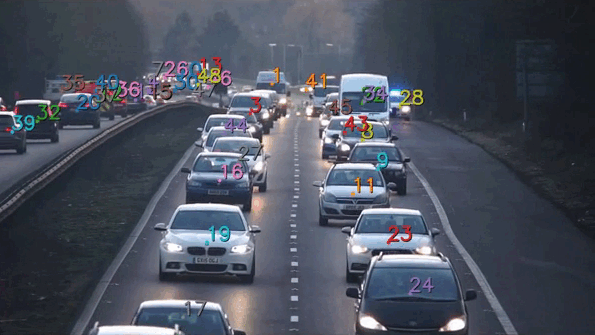
\includegraphics[scale=0.35]{cars.png}

\href{https://drive.google.com/file/d/1x0Y_jIFEGzIxii0dknu8mWWziKoa_wCL/view?usp=drive_link}{Полное видео с машинками.}

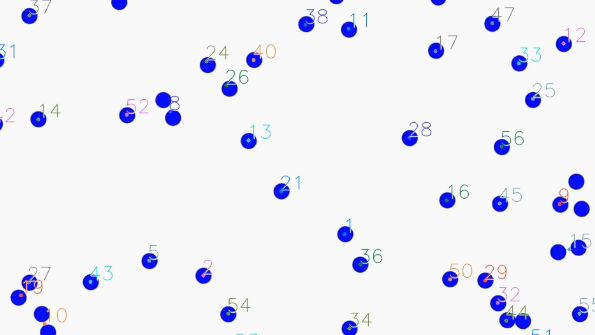
\includegraphics[scale=0.35]{white.png}

\href{https://drive.google.com/file/d/16_cmGNeH45PxP-VW5EQzEFFCMhzUTwx8/view?usp=drive_link}{Полное видео с точками.}
